\ifdefined\chinchin
	\documentclass[12pt, orivec]{extarticle} % 12pt, 14pt, 17pt, 20pt
\else
	\documentclass[10pt, orivec]{extarticle} % 12pt, 14pt, 17pt, 20pt
\fi
\usepackage{parskip}
\usepackage{amsmath}
\usepackage{amssymb}    % for \rightsquigarrow
\usepackage{wasysym}	% for frown face
\usepackage{mathrsfs} 	% for \mathscr
\usepackage{stmaryrd}
% \usepackage{unicode-math}
\usepackage[many]{tcolorbox}
\usepackage{ulem}
\usepackage{tikz-cd}		% commutative diagrams
\usepackage{tikz}
\usepackage{amsthm}
\usepackage{enumitem}	% for \ietemize custom labels
\usepackage{turnstile}	% longer turnstiles
\usepackage[sf,bf,big,raggedright,compact]{titlesec}	% change section color to blue
\usepackage{graphicx}	% Allows including images
% \usepackage[backend=biber,bibstyle=authoryear,citestyle=../authoryearbrack]{biblatex}
% \bibliography{../AGI-book}

\newtheorem{theorem}{Theorem}

\ifdefined\chinchin
	\newcommand{\cc}[2]{#1}
	\usepackage[CJKspace]{xeCJK}
	%\setCJKmainfont[BoldFont=SimHei,ItalicFont=AR PL KaitiM GB]{Alibaba PuHuiTi}
	\setCJKmainfont[Path={/usr/share/fonts/truetype/Alibaba PuHuiTi/}, BoldFont=Alibaba_PuHuiTi_Regular.ttf, ItalicFont=ukai.ttc]{Alibaba_PuHuiTi_Light.ttf}
	% \setmainfont[ItalicFont=Latin Modern Roman Slanted]{Alibaba Sans:style=Light}
\else
	\newcommand{\cc}[2]{#2}
	% \usepackage[no-math]{fontspec}
	% \setmainfont[Path={/usr/share/fonts/opentype/Alibaba Sans/},
	% BoldFont=Alibaba_Sans_Regular.otf,
	% ItalicFont=Alibaba_Sans_Light_Italic.otf]
	% {Alibaba_Sans_Light.otf}
	%\setmainfont{AlibabaSans_Light.otf}
	%\renewcommand{\baselinestretch}{0.8}
\fi

%\setlength{\headheight}{0cm}
%\setlength{\hoffset}{0cm}
%\setlength{\topmargin}{-2cm}
%\setlength{\oddsidemargin}{-2cm}
%\setlength{\evensidemargin}{-2cm}
%\setlength{\textwidth}{20cm}
%\setlength{\textheight}{26cm}
%\setlength{\headsep}{0.5em}
%\setlength{\topskip}{0.5em}
%\setlength{\footskip}{0.9cm}  % between bottom of page and page number
%\setlength{\floatsep}{0cm}
%\setlength{\textfloatsep}{0.6cm}
%\setlength{\intextsep}{0.5cm}
%\setlength{\parindent}{0em}   % em = width of capital M
%\setlength{\parskip}{10pt plus 5pt}

% Fix spilling of titles in bibliography:
%\DeclareFieldFormat*{title}{#1}
%
%\DeclareFieldFormat*{titlecase}{%
%    \ifdef{\currentfield}
%      {\ifcurrentfield{title}
%         {\usefield{\uline}{\currentfield}}%
%         {#1}}
%      {#1}}

\setcounter{secnumdepth}{1}		% 0 = no section numbers

\titleformat{\section}[hang]{\bfseries\Large\color{blue}}{\thesection \hspace{20pt}}{0pt}{}
\titleformat{\subsection}[hang]{\bfseries\large\color{blue}}{\thesubsection \hspace{10pt}}{0pt}{}
\titleformat{\subsubsection}[hang]{\bfseries\color{blue}}{}{0pt}{}

\itemsep1em
% \setlist[itemize]{noitemsep, topsep=15pt, partopsep=10pt}
\setlist[itemize]{topsep=15pt, partopsep=10pt}
\renewcommand{\labelitemi}{\textbullet}

\let\varzero\emptyset
\let\emptyset\varnothing		% round empty set
\newcommand{\vect}[1]{\symbf{#1}}
\newcommand{\book}[1]{$\NewSym[0.4]{../book-icon.png} \quad$ \parbox{0.9\textwidth}{\footnotesize #1}}
\newcommand{\code}[1]{{\small{\ttfamily #1}}}
\newcommand{\tab}{\hspace*{2cm}}
\newcommand{\powerset}{\raisebox{.15\baselineskip}{\Large\ensuremath{\wp}}}
\newcommand{\Chi}{\raisebox{2.5pt}{$\chi$}}
\newcommand*\KB{\vcenter{\hbox{
\includegraphics{../KB-symbol.png}}}}
\newcommand*\NewSym[2][0.5]{\vcenter{\hbox{\includegraphics[scale=#1]{#2}}}}
\newcommand*\sigmoid{\vcenter{\hbox{
\includegraphics{../sigmoid3.png}}}}
\newcommand{\smbox}[1]{\boxed{\footnotesize{\mbox{#1}}}}

\newcommand{\tikzmark}[1]{\tikz[overlay,remember picture] \node (#1) {};}

\newcommand{\Dfrac}[2]{%
\ooalign{%
      $\genfrac{}{}{2.9pt}0{\hphantom{#1}}{\hphantom{#2}}$\cr%
      $\color{white}\genfrac{}{}{1.5pt}0{\hphantom{#1}}{\hphantom{#2}}$\cr%
      $\color{white}\genfrac{}{}{1pt}0{\color{black}#1}{\color{black}#2}$}}

% \renewcommand{\thefootnote}{\fnsymbol{footnote}}
%\usepackage{perpage}
%\MakePerPage{footnote}
%\renewcommand{\thefootnote}{\ifcase\value{footnote}\or{*}
%	\or{$\dagger$}\or{**}\or{$\ddagger$}\fi}
%\renewcommand{\thefootnote}{\arabic{footnote}}
%\setcounter{footnote}{0}

\usepackage[hang,flushmargin]{footmisc}
\interfootnotelinepenalty=10000

% \usepackage[no-math]{fontspec}
% \setmainfont[BoldFont=Alibaba_Sans_Regular.otf,ItalicFont=Alibaba_Sans_Light_Italic.otf]{Alibaba_Sans_Light.otf}

\usepackage[backend=biber]{biblatex}
\bibliography{../AGI-book}

\usepackage[active,tightpage]{preview}		% for continuous page(s)
\renewcommand{\PreviewBorder}{0.5cm}
\renewcommand{\thempfootnote}{\arabic{mpfootnote}}

\usepackage[absolute,overlay]{textpos}		% for page number on upper left corner

\usepackage{color}
% \usepackage{mathtools}
\usepackage[hyperfootnotes=false]{hyperref}

% \usepackage[backend=biber,style=numeric]{biblatex}
% \bibliography{../AGI-book}
% \renewcommand*{\bibfont}{\footnotesize}

\usetikzlibrary{shapes}
% \usepackage[export]{adjustbox}	% ??
\usepackage{verbatim} % for comments
% \usepackage{newtxtext,newtxmath}	% Times New Roman font

\titleformat{\section}[hang]{\bfseries\large\color{cyan}}{}{0pt}{}
% \numberwithin{equation}{subsection}

\newcommand{\underdash}[1]{%
	\tikz[baseline=(toUnderline.base)]{
		\node[inner sep=1pt,outer sep=10pt] (toUnderline) {#1};
		\draw[dashed] ([yshift=-0pt]toUnderline.south west) -- ([yshift=-0pt]toUnderline.south east);
	}%
}%

\newcommand\reduline{\bgroup\markoverwith{\textcolor{red}{\rule[-0.5ex]{2pt}{0.4pt}}}\ULon}

%\DeclareSymbolFont{symbolsC}{U}{txsyc}{m}{n}
%\DeclareMathSymbol{\strictif}{\mathrel}{symbolsC}{74}
%\DeclareSymbolFont{AMSb}{U}{msb}{m}{n}
%\DeclareSymbolFontAlphabet{\mathbb}{AMSb}
%\setmathfont{lmroman17-regular.otf}
\DeclareMathOperator*{\argmin}{arg\,min}
\DeclareMathOperator*{\argmax}{arg\,max}

% \usepackage[most]{tcolorbox}
%\tcbset{on line,
%	boxsep=4pt, left=0pt,right=0pt,top=0pt,bottom=0pt,
%	colframe=red,colback=pink,
%	highlight math style={enhanced}
%}
%\newcommand{\atom}{\vcenter{\hbox{\tcbox{....}}}}

\let\oldtextbf\textbf
\renewcommand{\textbf}[1]{\textcolor{cyan}{\oldtextbf{#1}}}

\newcommand{\logic}[1]{{\color{violet}{\textit{#1}}}}
\newcommand{\underconst}{\includegraphics[scale=0.5]{../2020/UnderConst.png}}
\newcommand{\KBsymbol}{\vcenter{\hbox{
\includegraphics[scale=1]{../KB-symbol.png}}}}
\newcommand{\token}{\vcenter{\hbox{\includegraphics[scale=1]{token.png}}}}
\newcommand{\proposition}{\vcenter{\hbox{\includegraphics[scale=0.8]{proposition.png}}}}

\begin{document}

\begin{preview}

\cc{
\title{\vspace{-1cm} \bfseries\color{cyan}{\Large Solidi 加密貨幣 - 白皮書}}
}{
\title{\vspace{-1cm} \bfseries\color{cyan}{\Large Solidi Coin - White Paper}}
}

% \cc{
% \author{YKY (甄景賢)}}{
% \author{YKY (Yan King Yin)}
% }

\date{\vspace{-1.5cm}{\small \today}} % Date, can be changed to a custom date

\cc{
\centerline{\includegraphics[scale=0.6]{凝聚力-logo-0.png}}
}{
\centerline{\includegraphics[scale=0.4]{Solidarity-logo-0.png}}
}

\maketitle

\setcounter{section}{-1}
\newcounter{mypage}
\setcounter{mypage}{0}

% (1) Circled page number on upper left corner
%\begin{textblock*}{5cm}(2.1cm,2.3cm) % {block width} (coords)
%{\color{red}{\large \textcircled{\small \themypage}}}
%\addtocounter{mypage}{1}
%\end{textblock*}

\begin{minipage}{\textwidth}
\setlength{\parskip}{0.4\baselineskip}

\section{\cc{Solidi 的貨幣經濟學\\}{Economics of the Solidi Coin \\}}

\begin{itemize}
\cc{
	\item Solidi 幣的特點 是以\textbf{投票}形式 賺取的,例如 在新聞平台上發評論,被 \textbf{點贊} 即能獲得 貨幣獎勵。幣值也稱爲 \textbf{聲譽},也等於 \textbf{投票權} (下述)。
}{
	\item Solidi coins are earned via \textbf{voting}.  For example, if your comment on a news site is liked by someone, you get rewarded with Solidi.  Coins are also synonymous with \textbf{reputation}, and also equivalent to \textbf{voting power} (explained below).
}

\cc{
	\item \textbf{指數式 兌換:}  用戶可以花錢買 聲譽/投票權,但所需的價錢 會隨着聲譽 \textbf{指數式}增加。 換句話說,即使最有錢的個人或基金,都無法用錢換取極大的聲譽值,這保障了 聲譽不會純粹被 資本 主導。也可以說 Solidi 跟現時世界上的 money 是不同類的一種價值,它可以糾正 貧富懸殊的 財富分配\footnote{譬如《正義》一書的作者、哈佛大學教授 Michael Sandel 說: 大部分人都很感激我們的中學、小學老師,而我們也欣賞 美斯 (Messi) 是世界足球明星,但 美斯 的薪金 卻是一般教師薪金 的好幾萬倍,這裏面似乎有點不妥。},因爲現時世界的財富分配 服從 log-normal distribution (對數-正態分佈)。 以下說「現金」泛指傳統金錢。
}{
	\item \textbf{Exponential Conversion.}  A member can spend money to ``pump up'' his reputation, but it gets \textbf{exponentially} more expensive as his reputation goes up.  % $e^{kR}$ is required to increase one unit of $R$, where $R$ is reputation, $k$ is a scaling constant, eg. $1/1000$.
	This prevents reputation from being dominated solely by capital, as even the wealthiest individuals or funds could not buy a lot of reputation.  In other words, Solidi is essentially different from traditional money;  It may correct the problem of unfair wealth distribution\footnote{As Michael Sandel, Harvard professor and author of the book ``Justice,'' says:  most of us are grateful to our high school teachers, and we also appreciate the soccer skills of Lionel Messi, but Messi's salary is many thousands of times that of a school teacher's, making us question that something may be wrong with our society.}, as current wealth in our world follows a log-normal distribution.  Below, ``cash'' refers to traditional money.
}

\cc{
	\item \textbf{提取款項:}  用 Solidi 兌換現金, 即上述的逆運算,則可以得到對數式的現金值。但這樣,當某會員得到了稍為可觀的聲譽,就很有可能 cash-out (withdraw),獲得現金,而導致平台因缺乏現金而崩盤。 解決辦法是: cash-out 是根據 整體 聲譽的 \textbf{比例} 計算的。 當現金儲備 (即傳統 money) 很少的時候,cash-out 微不足道。 用一句口號概括就是:「指數式買入、線性賣出」
}{
	\item \textbf{Withdrawals} is the reverse of the above, but this may be problematic.  As some users get considerable reputation, they may be tempted to cash-out (withdraw), causing the platform to run out of cash and collapse.  How to prevent this?  A solution is to calculate withdrawal as a \textbf{proportion} of the reputation pool.  This means that when the total cash reserve of the platform is low, withdrawals are also insignificant.  In slogan this may be summarized as: \textit{buy exponentially, sell proportionately}.
}

\cc{
	\item \textbf{Solidi 的慷概性:}  賺取 聲譽 是很容易的,例如,每次 ``like'' 別人的評論,則評論者獲得 +1 聲譽值,而點贊者 扣除 $\frac{1}{100}$ 聲譽值。 因此人們不會吝嗇 給別人點贊。
}{
	\item \textbf{Generosity of Likes.}  Every time a member likes a comment, the creator of the comment get +1 unit reputation, while the sender gets $\frac{1}{100}$ deduction in reputation.  This encourages users not to be stingy with likes.
}

\cc{
	\item 我們的 \textbf{核心價值} 是:
	\begin{equation} \nonumber
		\vcenter{\hbox{\includegraphics[scale=0.7]{DAO-核心價值.png}}}
	\end{equation}
	這些都是很經典的價值,在世界各地的文化裏都有其雛形,但在西方 啓蒙時代 系統性地提出,這並不表示盲目崇拜西方思想。 隨着科技進步,以上這些原則都是 \textbf{可驗證的} (verifiable),例如 區塊鏈、開源軟件 等都是可驗證的。
}{
	\item Our \textbf{Core Values} are:
	\begin{equation} \nonumber
		\vcenter{\hbox{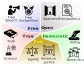
\includegraphics[scale=0.7]{DAO-principles.png}}}
	\end{equation}
	These are all very classical ideas developed in the Enlightenment period in the West, but are increasingly promoted as ``universal'' as they have primitive roots in almost every culture.  It does not mean imposing Western values on the rest of the world.  As our technology progresses, all these notions can now be \textbf{verifiable}, eg. blockchains and open-source.
}

\cc{
	\item \textbf{聲譽 有什麼價值?} 某個領域的專家,在別的領域不一定是專家,所以「聲譽」必需以不同的 領域 劃分。 我們希望 Solidi 平台完全是由 民主 的方式運行的,也就是說,以 \textbf{加權投票} 決定平台的發展方向,而 權重 就是聲譽值。 但 投票權 並不僅限於 Solidi 平台, 它可以發展到 任何領域,包括: 商業、科技、政治活動 (political activism).  很多人不明白 爲什麼 賺錢 要牽涉政治,其實在所有發展中國家(例如非洲),不完善的政治 institutions 是 阻礙 經濟發展的主要原因,包括各種 \textbf{貪腐},導致經濟 停滯不前 甚至倒退。 後發展的人民必需改變政治制度,而 Solidi 平台是爲 全世界的 後發展國家 邁出的一步。
}{
	\item \textbf{What is the economic value of Reputation?}  Expertise in one domain does not imply it in other domains;  so Reputation should be classified by domain.  We intend the Solidi platform to operate strictly by democracy, ie. via \textbf{weighted voting} where weights are reputation.  But Reputation need not be confined to the Solidi platform;  it extends to other domains such as:  business, technology, and political activism.  Many people don't understand why business should involve politics, but the lack of well-functioning political institutions in developing countries is a major obstacle to their economic development.  This includes various forms of \textbf{corruption}.  The people of developing nations must strive to reform our political institutions, and Solidi is a step towards this direction.
}
\end{itemize}

\end{minipage}
\end{preview}

\begin{preview}
%\begin{textblock*}{5cm}(2.1cm,2.3cm) % {block width} (coords)
%{\color{red}{\large \textcircled{\small \themypage}}}
%\addtocounter{mypage}{1}
%\end{textblock*}
\begin{minipage}{\textwidth}
\setlength{\parskip}{0.4\baselineskip}

Some formulas:
\begin{itemize}
	\item \textbf{To buy} $N$ Solidi with cash $W$:\\
		\begin{equation}
		W = e^{k \cdot N}
		\end{equation}
	where $k$ is a conversion constant such as 1000. \\
	For example, with US\$100, one can buy

	\item \textbf{To sell} $m$ Solidi, withdrawing cash $W$.  Suppose the whole platform has a total of $N$ Solidi (generated by mutual ``liking'').  Suppose the actual cash pool of the Solidi platform is $T = e^{k \cdot n}$, in other words, $n$ Solidi.  We cannot simply let users withdraw $W = e^{k \cdot m}$ as that would eventually bankrupt the platform.  Instead we will let him withdraw, proportionately,
	\begin{equation}
		W = e^{k \cdot m \frac{n}{N}} .
	\end{equation}

\end{itemize}

\end{minipage}
\end{preview}

\end{document}
